\documentclass[12pt,a4paper]{article}

% Encoding and language
\usepackage[utf8]{inputenc}
\usepackage[T1]{fontenc}
\usepackage[english]{babel}
\usepackage{subcaption}

\usepackage{float}
\usepackage{booktabs}
\usepackage{tabularx}
\usepackage{array}

\newcolumntype{C}[1]{>{\centering\arraybackslash}p{#1}}
\newcolumntype{L}[1]{>{\raggedright\arraybackslash}p{#1}}

\usepackage[most]{tcolorbox}
\usepackage{enumitem}
\usepackage{parskip}
\usepackage[a4paper,margin=1in]{geometry}

% Page layout
\usepackage[a4paper,margin=1in]{geometry}
\usepackage{setspace}
\onehalfspacing
\usepackage{parskip}

% Math
\usepackage{amsmath,amssymb,amsthm}

% Tables and figures
\usepackage{graphicx}
\usepackage{booktabs}
\usepackage{longtable}
\usepackage{array}
\usepackage{float}
\usepackage{caption}
\usepackage{subcaption}

% Links and references
\usepackage[hidelinks]{hyperref}
\usepackage[nameinlink,noabbrev]{cleveref}

% Lists
\usepackage{enumitem}

% Optional useful packages
\usepackage{xcolor}
\usepackage{pdflscape}
\usepackage{multirow}

\begin{document}

\title{Master's Thesis}
\author{Your Name}
\date{\today}

\maketitle

\section{Motivation}

\subsection{The recent boom in AI stocks and concentration risk}

Over the past three years, the U.S.\ stock market has increasingly come to reflect investor enthusiasm about artificial intelligence. What began as broad interest in a promising new technology evolved into one of the most concentrated equity rallies in recent history. The public release of ChatGPT on November 30, 2022, did not create this trend on its own, but it became a visible turning point in market narratives around generative AI and was followed by a marked revaluation of firms perceived to be central to the AI economy.

At the centre of this revaluation are seven large-capitalisation technology firms, collectively known as the Magnificent Seven: Apple, Amazon, Alphabet, Meta Platforms, Microsoft, Nvidia, and Tesla. These companies, all of which are widely viewed as builders, deployers, or enablers of AI infrastructure, have dramatically outperformed the rest of the market since late 2022. Figure~\ref{fig:mag7_vs_sp500} illustrates this development. The figure plots the cumulative return of three portfolios from January 2021 through April 2026: an equal-weighted portfolio of the Magnificent Seven, the S\&P 500 index, and the S\&P 500 with the Magnificent Seven removed. Before the release of ChatGPT, the three portfolios moved broadly together, including through the sharp drawdown of 2022. The divergence begins in late 2022 and accelerates throughout 2023 and 2024. By early 2026, the Magnificent Seven had gained approximately 200 percent relative to the start of 2021, compared with around 80 percent for the S\&P 500 as a whole. The remaining 493 companies in the index returned roughly 50 percent. In other words, a large share of the headline index performance over this period was driven by a very small number of firms.

\begin{figure}[H]
    \centering
    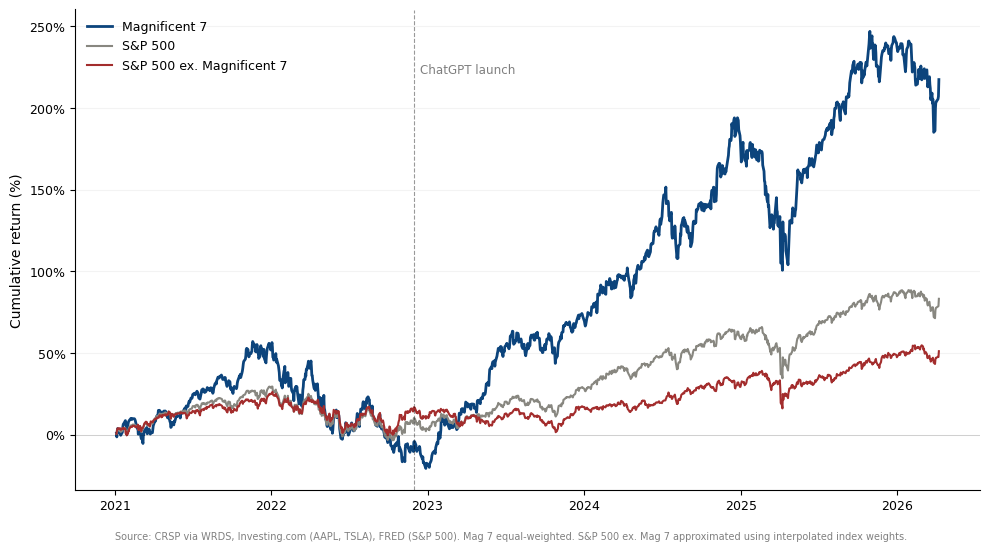
\includegraphics[width=\textwidth]{Pics/Mag7 & SP500.png}
    \caption{Cumulative returns: Magnificent 7 (equal-weighted) vs.\ S\&P 500 vs.\ S\&P 500 ex.\ Magnificent 7, January 2021 to April 2026. Sources: CRSP via WRDS, Investing.com, FRED.}
    \label{fig:mag7_vs_sp500}
\end{figure}

According to analysis by M\&G Investments, roughly 70 percent of the approximately \$24 trillion in market value added to the S\&P 500 since ChatGPT's launch can be attributed to companies linked to AI infrastructure and semiconductors, with around 65 percent of the total index rise coming from just ten stocks.\footnote{Vine, C., ``AI: Bubble or bottleneck?'', M\&G Investments, December 2025.} Vontobel Asset Management similarly reports that just 42 AI-related stocks accounted for more than half of total market returns since the launch of ChatGPT.\footnote{Souccar, D., ``What we don't know: the gap between AI hype and economic reality'', Vontobel Asset Management, February 2026.} 

The degree of concentration is unusual in historical context. At the start of 2015, the Magnificent Seven collectively represented roughly 12 percent of the S\&P 500's total market capitalisation. By the end of 2025, that share had risen to more than 34 percent, meaning that seven firms out of five hundred accounted for more than one third of the index.\footnote{``Should Investors Be Worried That the Magnificent Seven Make Up 35\% of the S\&P 500?'', Motley Fool Research Report, via Nasdaq, January 2026.} Market breadth has also narrowed considerably. In 2023 and 2024, fewer than 28 percent of S\&P 500 constituents outperformed the index, the narrowest breadth since at least 1995.\footnote{First Trust Advisors / Capital IQ, cited in ``S\&P 500 Q3 performance check'', Proactive Advisor Magazine, October 2025.} For the hundreds of millions of investors around the world who hold passive exposure to the S\&P 500 through index funds and pension products, returns have therefore become unusually dependent on the valuation of a small number of technology firms.

Figure \ref{fig:Mag 7 Share of SP500} shows that this was not only a story of strong returns, but also of rising index concentration. Over the past decade, the combined market capitalisation of the Magnificent Seven increased sharply both in absolute terms and as a share of the S\&P 500. What had been a large but manageable group of firms in the mid-2010s gradually came to dominate the index, with their combined weight rising from around the low teens to more than one third of total market capitalisation by 2025--2026. This is important because it means that the recent AI rally did not simply lift a handful of stocks; it also changed the structure of the market itself. As the weight of these firms increased, the performance of the S\&P 500 became increasingly tied to the valuation of a very small group of companies, all heavily linked to the same technological narrative.

\begin{figure}[H]
    \centering
    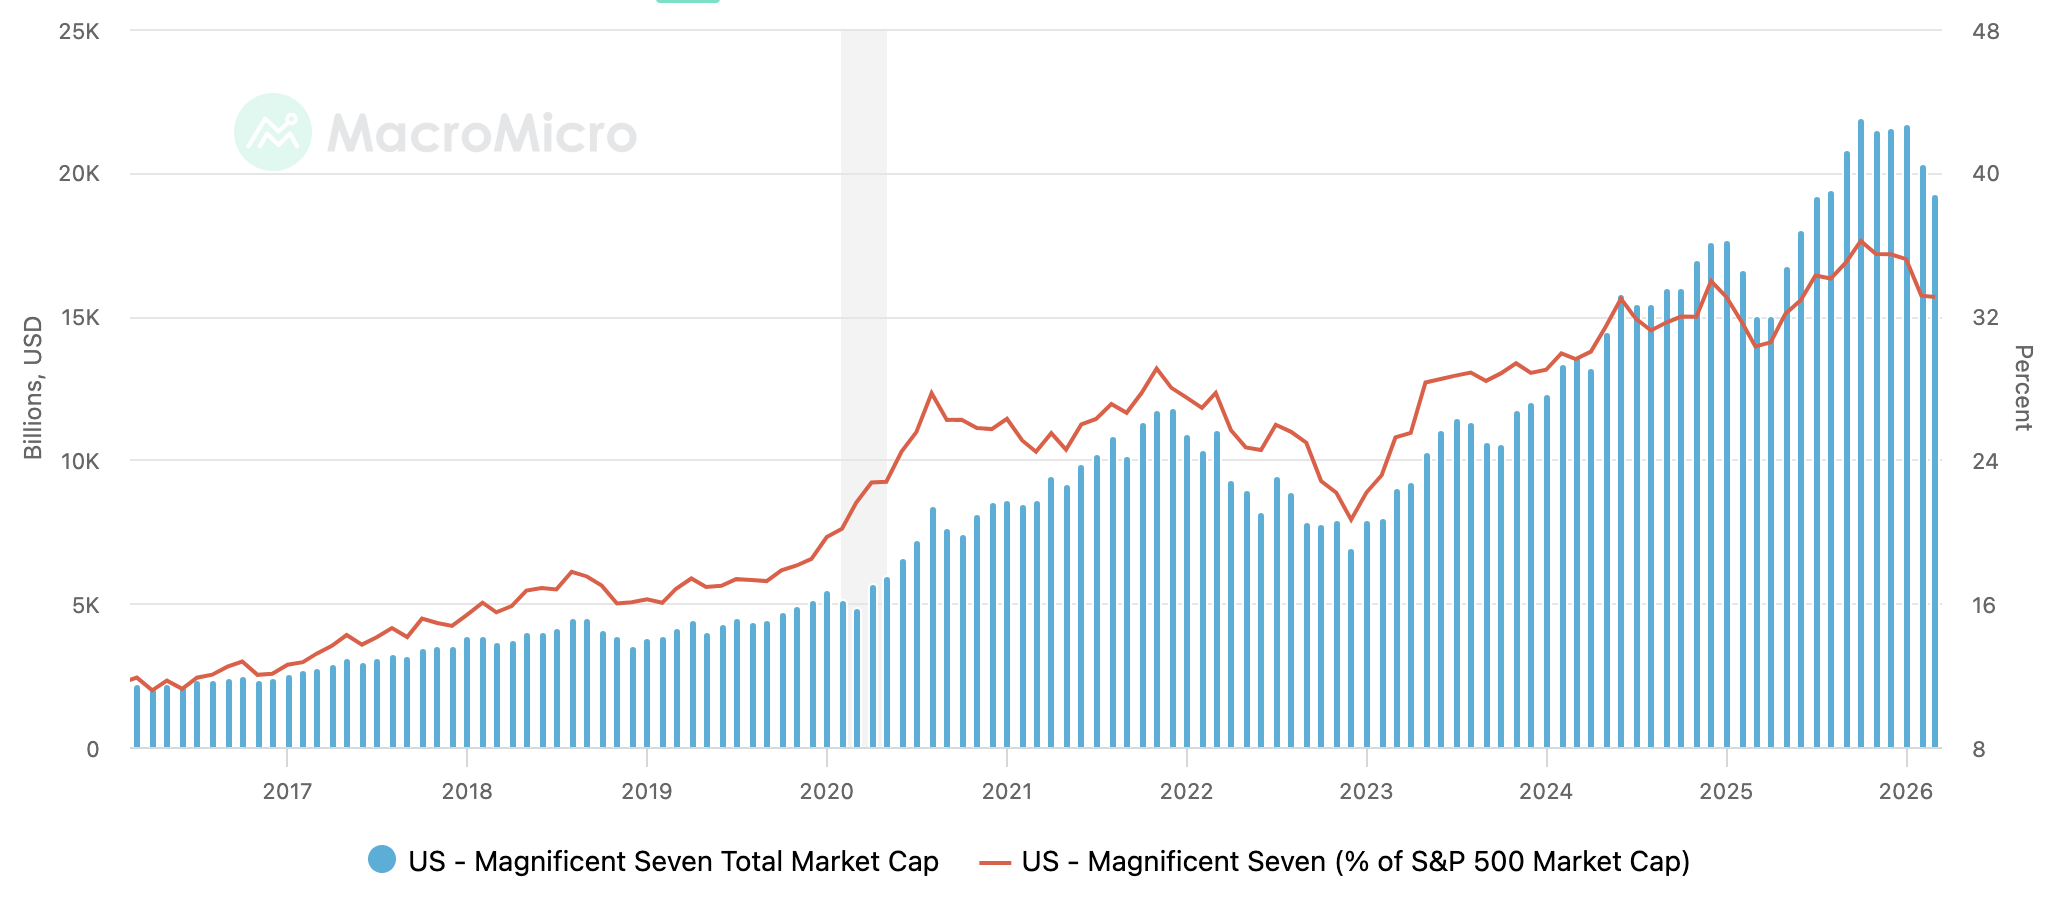
\includegraphics[width=\textwidth]{Pics/Mag7 share og sp500.png}
    \caption{Combined market capitalisation of the Magnificent Seven and their share of total S\&P 500 market capitalisation, 2016--2026. MacroMicro}
    \label{fig:Mag 7 Share of SP500}
\end{figure}


This concentration also introduces substantial downside risk. During the 2022 sell-off, the Magnificent Seven declined by approximately 41 percent, roughly double the S\&P 500's 20 percent decline.\footnote{``The Magnificent Seven's Market Cap vs.\ the S\&P 500'', Motley Fool, April 2026.} The same mechanism that amplifies gains during a rally can also magnify losses when sentiment turns, especially when the rally is closely tied to a single investment theme.

That theme is the expectation that artificial intelligence will reshape the global economy. The companies driving the rally are also the firms most directly associated with AI. Nvidia, which designs the processors used to train and run large language models, saw its stock price increase by a factor of twelve between January 2023 and December 2025.\footnote{Author's calculation based on CRSP daily return data via WRDS.} Meta and Alphabet experienced sharp re-ratings as investors attached greater value to the potential of AI in advertising and cloud services. Microsoft, through its partnership with OpenAI, became one of the clearest corporate symbols of the generative AI wave. Exposure to artificial intelligence has therefore been treated by markets not merely as a positive attribute, but increasingly as a defining valuation narrative.

Whether this response is proportionate remains an open question. Behind the surge in equity valuations lies an equally striking surge in corporate capital expenditure. The largest technology companies have committed to AI-related infrastructure investment on a scale with little recent precedent, with hundreds of billions of dollars flowing into data centres, semiconductors, and power generation capacity. It is to this investment boom, and the questions it raises about fundamentals, expectations, and market risk, that we now turn.

A useful way to frame the current episode is to compare it with the dot-com boom. As Figures~\ref{fig:dotcom_price_earnings} and~\ref{fig:ai_price_earnings} show, the late-1990s rally was characterised by stock prices rising far faster than the earnings outlook of the leading firms, whereas in the current AI episode the rise in the share prices of major AI-exposed companies has to a greater extent been accompanied by stronger earnings growth. This does not imply that current valuations are necessarily justified. Earnings projections may still embed overly optimistic assumptions about adoption, monetisation, and future market power. But when assessing whether we are repeating history by over assessing the potential of new technology, this could ease our minds.

\\

\begin{figure}[H]
    \centering
    \begin{subfigure}[t]{0.49\textwidth}
        \centering
        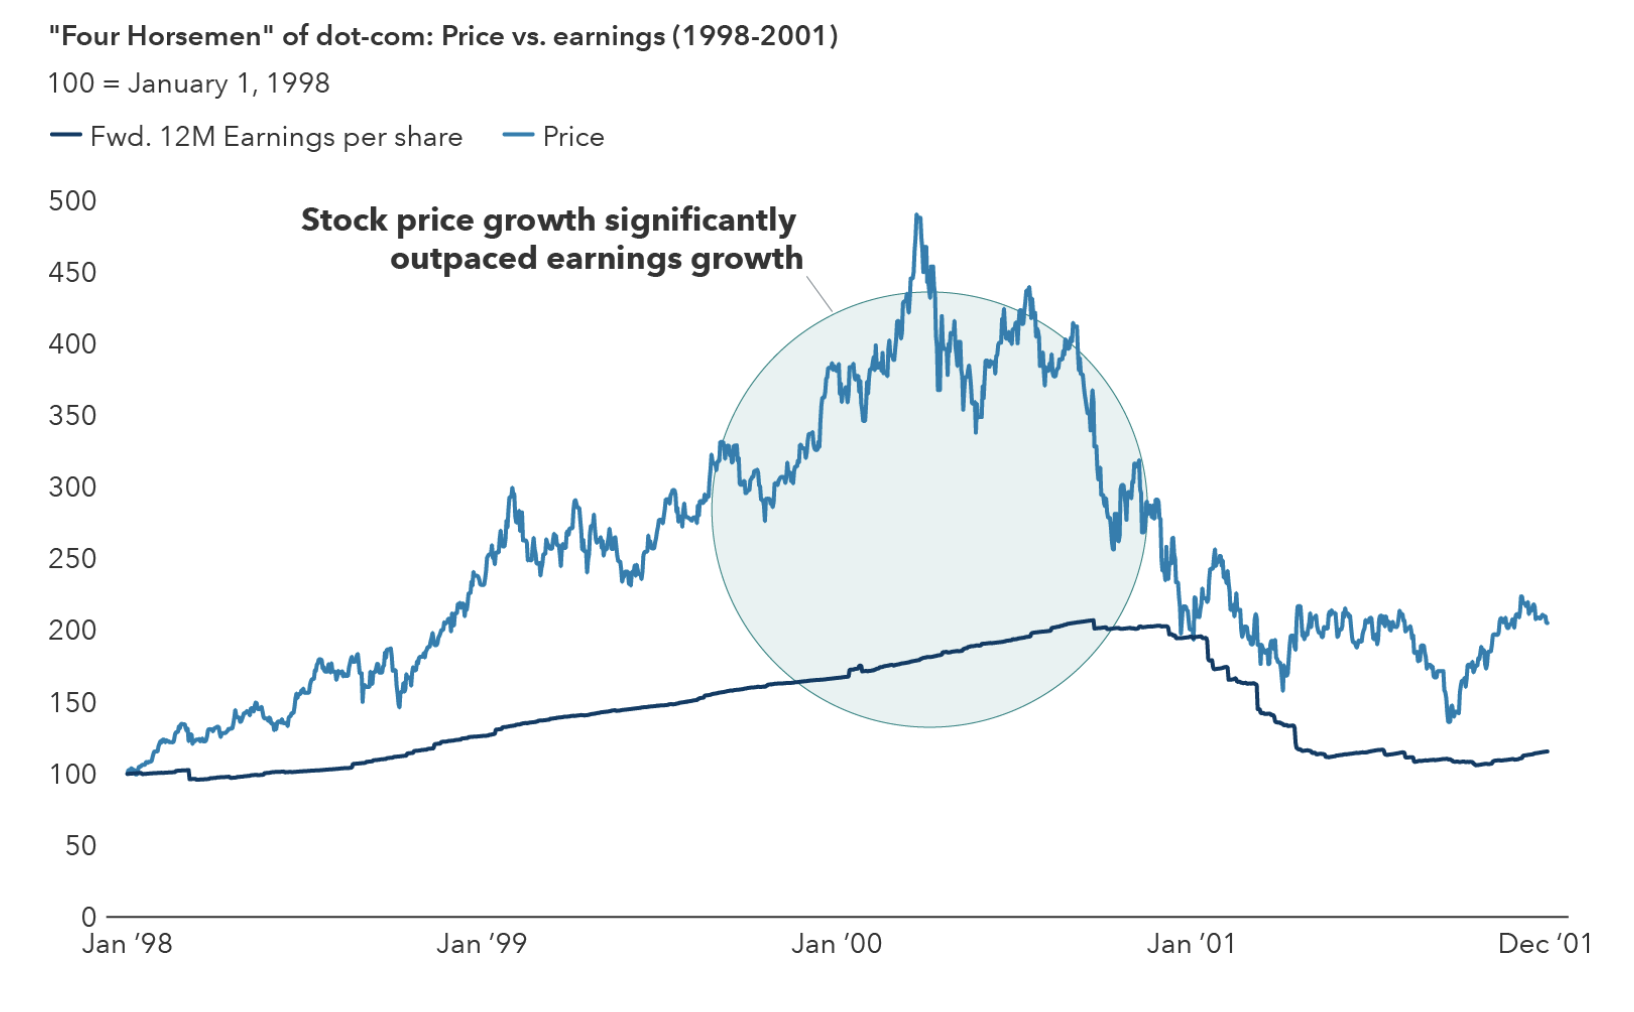
\includegraphics[width=\textwidth]{Pics/PE dot-com.png}
        \caption{Dot-com era}
        \label{fig:dotcom_price_earnings}
    \end{subfigure}
    \hfill
    \begin{subfigure}[t]{0.49\textwidth}
        \centering
        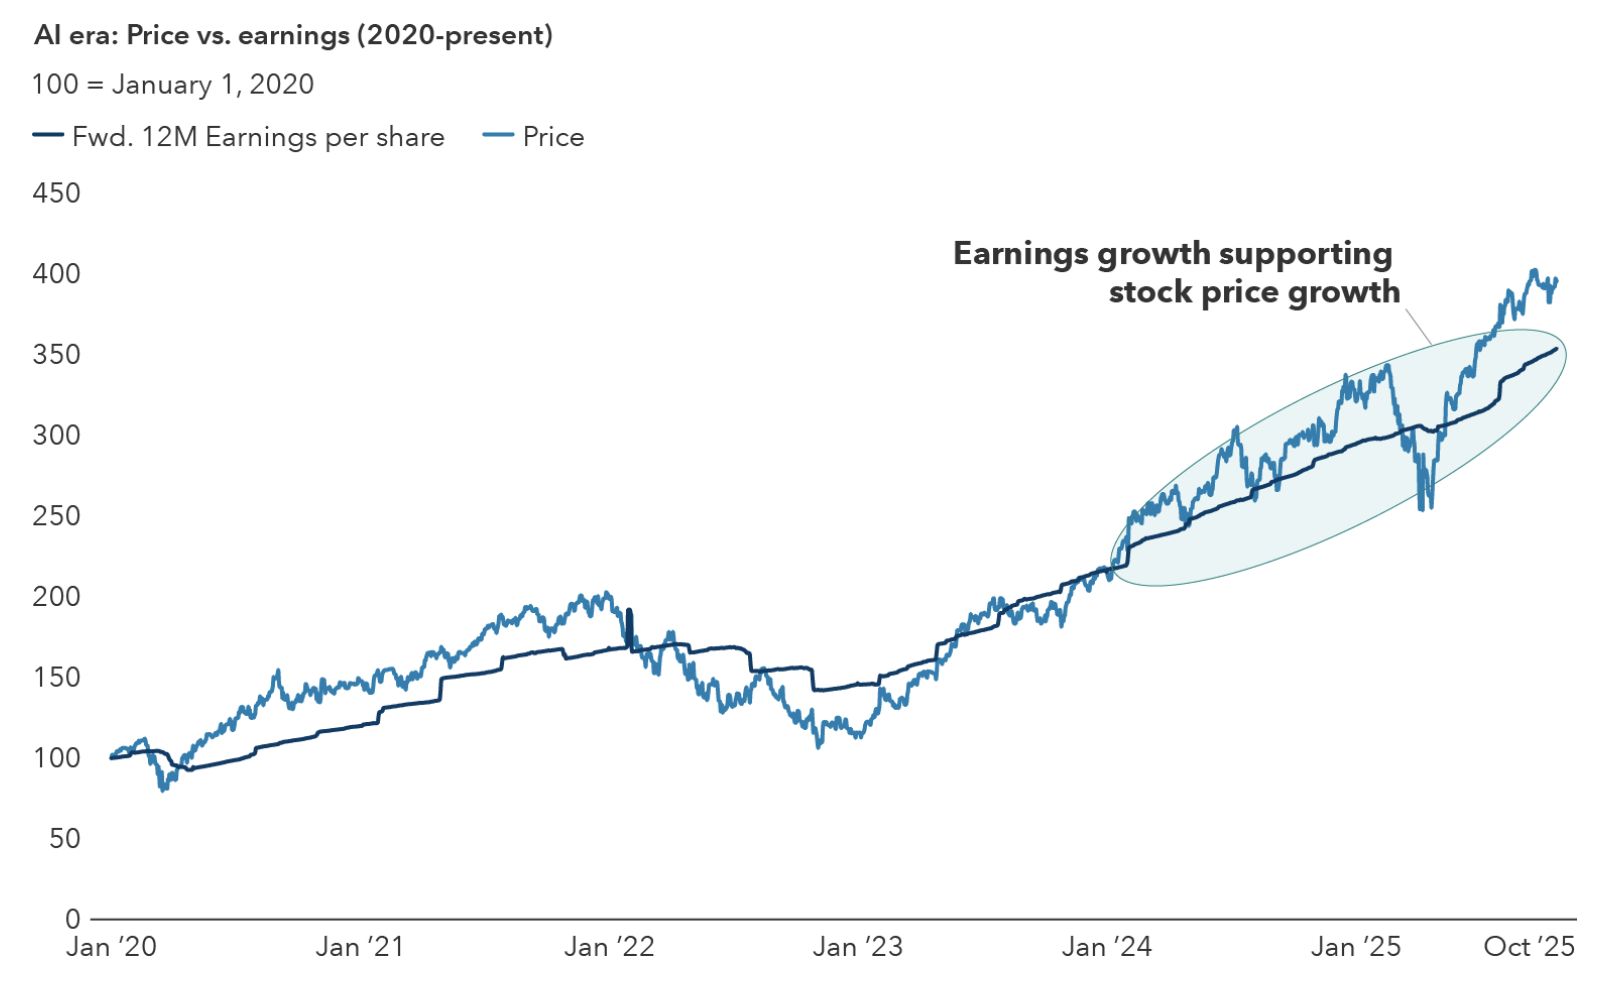
\includegraphics[width=\textwidth]{Pics/PE now.png}
        \caption{AI era}
        \label{fig:ai_price_earnings}
    \end{subfigure}
    \caption{Stock prices and forward earnings in the dot-com era and the current AI era.}
    \label{fig:price_earnings_comparison}
\end{figure}

\\

Figure~\ref{fig:NASDAQ Price Return} reinforces the point that the current AI rally, while unusually strong, has not yet reached the same degree of market excess as the final phase of the dot-com boom. The Nasdaq rose much more violently in the run-up to March 2000, suggesting a faster and broader detachment of prices from fundamentals than has so far been observed in the present boom. 

\begin{figure}[H]
    \centering
    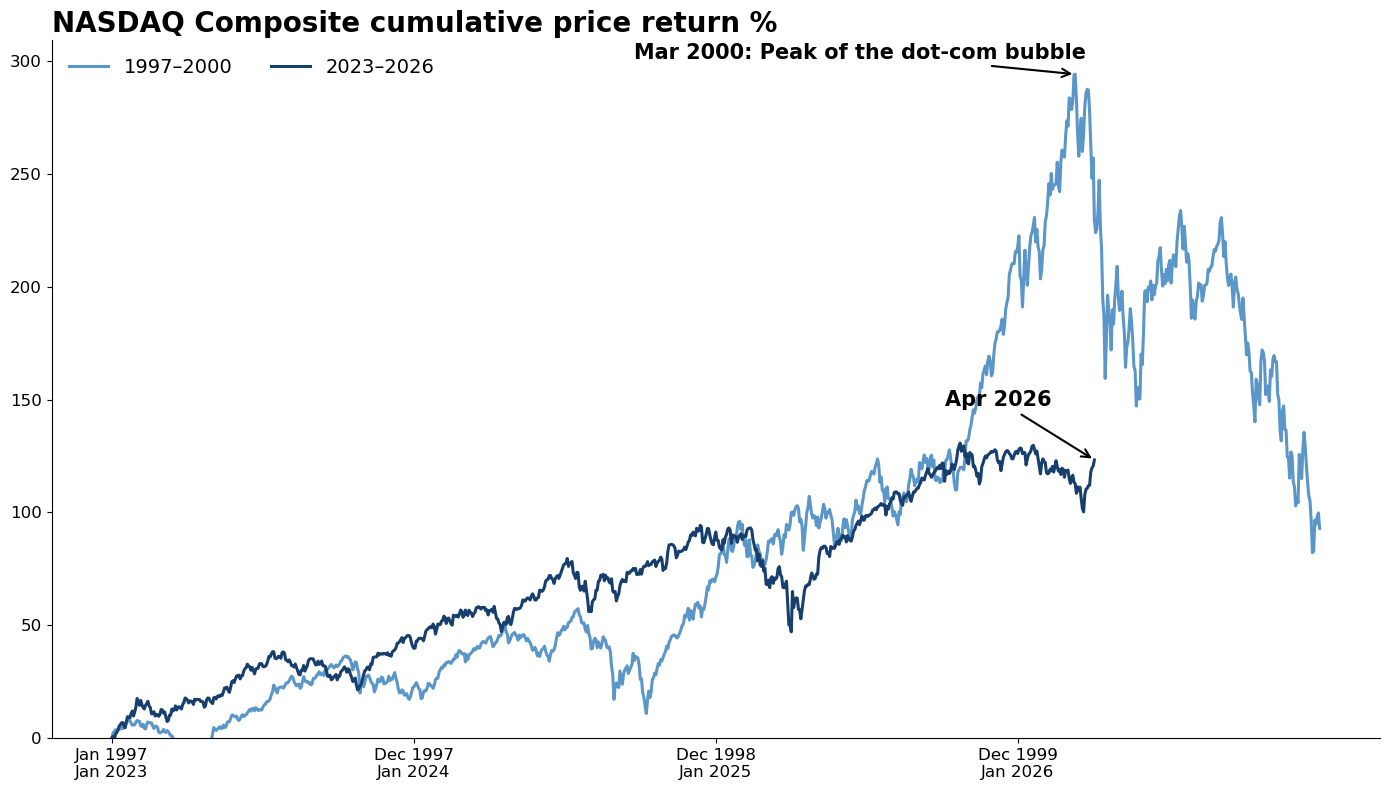
\includegraphics[width=\textwidth]{Pics/NASDAQ Price Return.png}
    \caption{Composite cumulative Price Return of Nasdaq, Dot-com era vs now. FRED Database, Own calculations}
    \label{fig:NASDAQ Price Return}
\end{figure}

An additional difference relative to the dot-com episode is that some of the most prominent firms associated with the current AI wave remain privately held. OpenAI, which played a central role in the renewed market enthusiasm surrounding generative AI after the release of ChatGPT in November 2022, is not publicly listed, and neither are several other high-profile AI firms. This matters because speculative dynamics often intensify when fast-growing firms become accessible to public equity investors. In the late 1990s, high-growth technology firms were able to attract large public valuations before profitability was firmly established. A similar pattern could emerge if leading AI startups eventually enter public markets. \footnote{Capital ideas: Are we in a Bubble?}

Whether the current market response is proportionate nevertheless remains an open question. Rising share prices and stronger earnings expectations suggest that the AI boom cannot be dismissed as a purely speculative episode. At the same time, valuations ultimately depend on whether the anticipated gains from artificial intelligence are matched by real economic investment and future returns. The next step is therefore to move from financial markets to the underlying corporate response. If firms themselves believe that AI will transform production, this should be visible not only in asset prices, but also in the scale and composition of their investment spending. 

\subsection{CAPEX spending}

The strong rise in AI-related stock prices naturally raises a deeper question: is this mainly a story about market excitement, or is something real also happening underneath? One way to get closer to that question is to look at what firms are actually doing with their money. If companies truly believe that artificial intelligence will change how business is done, then that belief should show up not only in share prices, but also in investment decisions.

Figure~\ref{fig:ai_capex} shows that this is exactly what we see. Capital expenditure among the largest technology firms has risen sharply, reflecting very large investments in data centres, semiconductors, and other infrastructure needed to develop and run AI systems. This matters because it suggests that the current AI boom is not just being driven by investors in financial markets. The firms at the centre of the story are also making large, concrete bets on AI themselves. In that sense, the figure points to something more substantial than a pure speculative narrative. 

\begin{figure}[H]
    \centering
    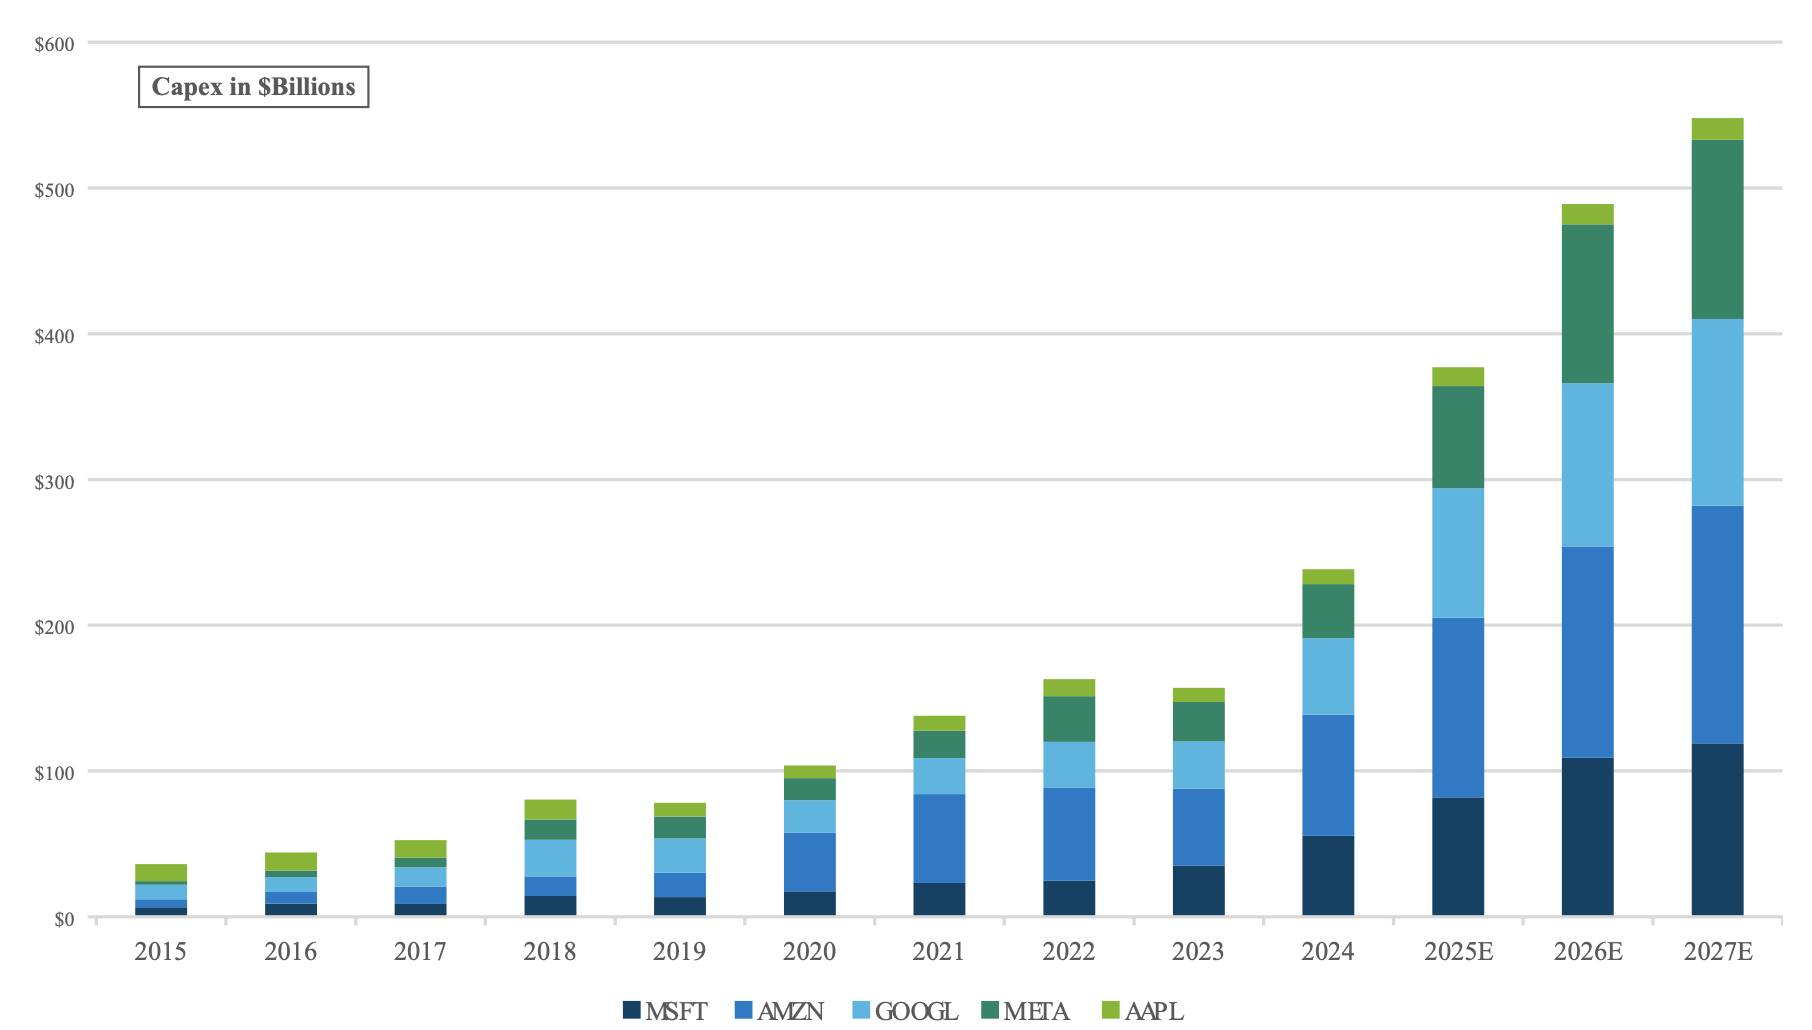
\includegraphics[width=\textwidth]{Pics/CAPEX.png}
    \caption{Capital expenditure among major technology firms, 2015--2027E. Source: SEC filings, FactSet consensus estimates, and reproduced from \textit{Built to Last? Understanding the Foundation Supporting the Growth of AI}.}
\label{fig:ai_capex}
\end{figure}

At the same time, the graph does not make the valuation question disappear. If anything, it makes it more important. Once firms begin spending at this scale, the success of the AI story depends not only on expectations, but on whether those investments eventually generate the profits, productivity gains, or cost savings that markets seem to anticipate.

The spending is concentrated among a remarkably small number of firms. Microsoft, Amazon, Alphabet, and Meta, the four largest hyperscalers, account for the vast majority of AI-related capital expenditure, and their announced plans continue to be revised upward. Capex projections for 2026 came in roughly 27 percent higher than projections made just a quarter earlier.\footnote{Payden \& Rygel, ``SaaS Stumble: Technology Software Stocks Versus Hyperscaler Capex Projection,'' Chart of the Week, February 6, 2026.} A McKinsey report from August 2025 projected \$6.7 trillion in global data centre buildout through 2030, equivalent to more than one percent of global GDP annually, with approximately 52 percent of this spending allocated to servers and chips.\footnote{McKinsey \& Company, ``The Data Center Balance Report,'' August 2025, cited in Mercer, ``AI Industry Review 2025,'' December 2025.} Meanwhile, Nvidia's sales surged from \$24 billion in 2021 to \$187 billion in 2025, driven almost entirely by demand for GPUs from these same hyperscalers.\footnote{Mercer, ``AI Industry Review 2025,'' December 2025. Nvidia sales figure based on Bloomberg data and Nvidia financial reports.} The infrastructure investment is therefore not only large in absolute terms but also highly concentrated in the same cluster of firms whose share prices dominate the S\&P 500.
 
An important counterargument to the view that this spending constitutes excessive risk is that, unlike in previous technology investment cycles, the current buildout has been largely self-financed. U.S. public technology companies have funded their AI capital expenditure almost entirely from free cash flow. As of late 2025, the ratio of aggregate free cash flow to capital spending among the top 3,000 U.S. stocks stood below one, meaning that firms were spending within their means. This stands in stark contrast to the dot-com era, when capital spending peaked at nearly four times free cash flow amid a debt-fuelled boom.\footnote{Ojjeh, A. and Fronczke, K., ``The New AI Playbook: Swapping Opex for Capex,'' Fidelity Investments, 2026. Based on Haver Analytics data as of December 31, 2025.} The Magnificent Seven have also seen a notable shift in cost structure: operating expenditure growth has slowed sharply while capex has accelerated, with the ratio of opex to capex falling from a long-run range of 2.5--4x to approximately 1.5x since mid-2024.\footnote{Ojjeh and Fronczke (2026), Exhibits 2 and 3. Based on Bloomberg Finance data as of September 30, 2025.} In one reading, this represents a rational substitution of labour costs for compute capacity, with firms spending less on headcount and more on infrastructure that may eventually do the work of the employees they are not hiring.
 
This view is further supported by the observation that return on invested capital among the largest AI-investing firms has remained resilient. Despite the sharp step-up in capex, ROIC for Meta and Alphabet has stayed above 30 percent for more than two consecutive years, suggesting that AI-driven productivity gains may already be helping to stabilise margins even as capital intensity rises.\footnote{Ojjeh and Fronczke (2026), Exhibit 4.} The current cycle also differs from the late-1990s internet buildout in one important respect. During the dot-com era, large volumes of fibre-optic cable, so-called ``dark fibre,'' were installed far ahead of actual demand, leading to years of idle capacity and poor returns on invested capital as telecom companies poured billions into infrastructure that sat unused. Eventually, capital markets shut down, driven by higher interest rates and a lack of near-term revenues. In the current AI cycle, GPUs have reportedly been deployed at or near full utilisation from day one, consistent with a pattern of demand pulling supply forward rather than supply racing ahead of demand.\footnote{Golan, J., ``Built to Last? Understanding the Foundation Supporting the Growth of AI,'' William Blair Investment Management, November 2025.}
 
However, these reassurances are not without qualification. The fact that current spending is self-financed does not mean that it will generate adequate returns. Free cash flow funding reduces the risk of a credit-driven collapse of the kind seen in 2000--2002, but it does not eliminate the risk of overinvestment. If the revenue that these investments are expected to generate does not materialise at the scale or pace that markets anticipate, the result would not be a wave of bankruptcies but rather a sustained period of compressed returns, asset writedowns, and downward pressure on the valuations of the firms at the centre of the index.
 
Several indicators suggest that the gap between investment and revenue remains wide. OpenAI, the most prominent model developer, has projected revenues rising from \$13 billion in 2025 to \$200 billion by 2030, an extraordinary growth trajectory, while simultaneously forecasting cumulative cash burn of approximately \$119 billion before reaching profitability in 2030.\footnote{OpenAI financial projections as reported by The Information, October 2025, cited in Mercer, ``AI Industry Review 2025,'' December 2025.} These projections embed highly optimistic assumptions about the pace at which enterprises and consumers will adopt and pay for AI services. If adoption is slower than expected, or if competition drives down pricing, as the emergence of efficient open-source models such as DeepSeek has begun to suggest, then the returns on the hundreds of billions of dollars in infrastructure now being built may fall substantially short of expectations.
 
During the telecom buildout of the late 1990s, fibre-optic infrastructure was installed on the assumption that bandwidth demand would grow exponentially. Demand did eventually materialise, and the infrastructure did eventually prove useful, but the lag between investment and payoff was long enough to destroy the firms that had financed the buildout.\footnote{Golan (2025).} The current AI infrastructure cycle avoids some of the worst features of that episode. The firms are profitable, the financing is internal, and utilisation rates are currently high. But it shares the same underlying vulnerability: the investment thesis depends on future demand materialising at a pace and scale that justifies present spending. If it does not, the market's current pricing of these firms will prove to have been too optimistic.

To investigate this, the next step is to define more precisely what it means for a firm to be exposed to artificial intelligence, and to construct a measure that allows us to compare outcomes across firms with different levels of AI engagement.

\section*{AI Dependency Grouping}

After examining the recent rise on the stock market of AI firms and the extent to which they leverage themselves, we want to look further into the major rise in market cap that these types of firms have seen in recent years. To do this there are many routes we can take, non of them perfect. We want to capture if there really have been an abnormal rise in these stocks, and what can explain this, but before we do that, we need to specify what it means to be an "AI company". Many firms in recent years have called themselves AI companies, and it has become synonymous with innovation and therefore a description that a lot of companies use. 

AI exposure is not a single observable variable. There is no objective measurment we can use, and no standard industry classificaion that seperates AI-dependent firms from the rest. Eisfeldt, Schubert, Taska and Zhang adresses this by mapping occupational exposure scores to firm level workforce data, but their apporach relies on data not publicly available. A more accessible approach is that of Ante and Saggu (2025), measuring how much firms themselves discuss AI in their regulatory fillings. This follow the logic: if a firm is reliant on artificial intelligence, it will show up more times in their filings than firms who is not reliant on artificial intelligence. 

Thereby, by counting the frequency of AI-related terms in 10-K filings, we can construct an ex-ante measure of AI engagement/dependency across out index. 

\subsection{Data and keyword selection}

The sample consists of all firms included in the S\&P 500 index as of 22 December 2022, the last available rebalancing date before year-end. The cutoff date of 31 December 2022 is chosen because it immediately precedes the period in which generative AI became a dominant market narrative. OpenAI released ChatGPT on 30 November 2022, and while the product attracted significant public attention within days, the broader repricing of AI-exposed equities unfolded primarily from early 2023 onward. By restricting the classification to information available before this date, the measure captures firms' pre-existing engagement with AI rather than their response to the boom itself — or the market's retrospective reinterpretation of which firms stood to benefit. Although ChatGPT was released on 30 November 2022, the 10-K filings retrieved under this cutoff were prepared and in most cases submitted before the product's launch. Annual reports reflect the fiscal year just ended and are drafted over a period of weeks to months; they cannot be meaningfully revised in response to a late-November event. The classification therefore captures pre-boom AI engagement despite the nominal overlap in calendar dates. An alternative cutoff of 31 December 2021 would avoid this overlap entirely but at the cost of relying on older filings that are less reflective of firms' AI positioning at the onset of the boom.

Three firms that subsequently failed during the banking turmoil of early 2023 are excluded (Silicon Valley Bank, Signature Bank, and First Republic Bank), as is one duplicate share class (Alphabet Class C, traded under the ticker GOOG). One additional firm, BlackRock, is excluded due to the volume of its regulatory filings rendering its 10-K inaccessible through the automated retrieval process. This leaves a final sample of 498 firms.

The AI exposure measure is based on a dictionary of eight terms: "artificial intelligence," "AI" (as a standalone word), "machine learning," "deep learning," "neural network(s)," "natural language processing," "computer vision," and "data science/scientist." Each term is unambiguously related to artificial intelligence or machine learning, and the list is informed by the keyword approach developed in Ante and Saggu (2025). Word-boundary matching is applied to "AI" to prevent false positives from common words containing the letters, and plural forms are captured where relevant. The choice to limit the dictionary to eight terms is deliberate. An initial screening of 65 candidate terms revealed that broader technology language, "automation," "algorithm," "cloud computing," "data center", appears frequently in 10-K filings but does not reliably distinguish AI-engaged firms from the rest. A utility company operating a data center or a bank describing its fraud-detection algorithms would score alongside NVIDIA and Alphabet, undermining the discriminating power of the measure. At the other end, terms that emerged primarily after the generative-AI boom  "large language model," "generative AI," "agentic", have near-zero frequency in pre-2023 filings and therefore contribute nothing to the cross-sectional variation. The eight retained terms capture the vast majority of meaningful AI-related disclosure while excluding both sources of noise.

\subsection{AI exposure score}

For each firm, the raw count of AI-related keyword appearances is divided by the total word count of the filing and multiplied by 10,000, producing a normalised AI exposure score expressed as mentions per 10,000 words. The normalisation is necessary because 10-K filings vary considerably in length, a 200-page filing will mechanically contain more of any term than a 50-page one, and without adjustment this would bias the measure toward firms with longer disclosures rather than firms with greater AI engagement.

The resulting distribution is heavily right-skewed. Of the 498 firms in the sample, 319 have zero AI-related mentions in their most recent pre-2023 filing. Among the remaining 179 firms, scores range from marginal to substantial. NVIDIA leads with 110 mentions and a normalised score of 22.49, more than double the next-highest firm, Hewlett Packard Enterprise (10.66). A cluster of semiconductor and software firms, including Intel, Adobe, Microsoft, IBM, and Juniper Networks, score in the 6-8 range, representing companies for which AI was already a meaningful part of the business narrative. Beyond this upper tail, scores decline rapidly: the median among mentioning firms is just 0.38. The left panel of Figure \ref{fig:ai_score_distribution} illustrates this distribution.

The right panel of Figure \ref{fig:ai_score_distribution} provides a point of comparison using the most recent available filings. The number of firms mentioning AI rose from 179 to 479, from roughly one-third to nearly the entire index. The distribution shifted substantially to the right, with the bulk of firms now scoring between 1 and 5, and the upper tail extending well beyond the pre-2023 maximum. Firms such as AMD, Adobe, and ServiceNow now reach scores above 30, a range that only NVIDIA occupied before the boom. This convergence supports the validity of the pre-2023 measure — the variation it captures has since compressed as AI disclosure became near-universal across the index.

\begin{figure}[H]
    \centering
    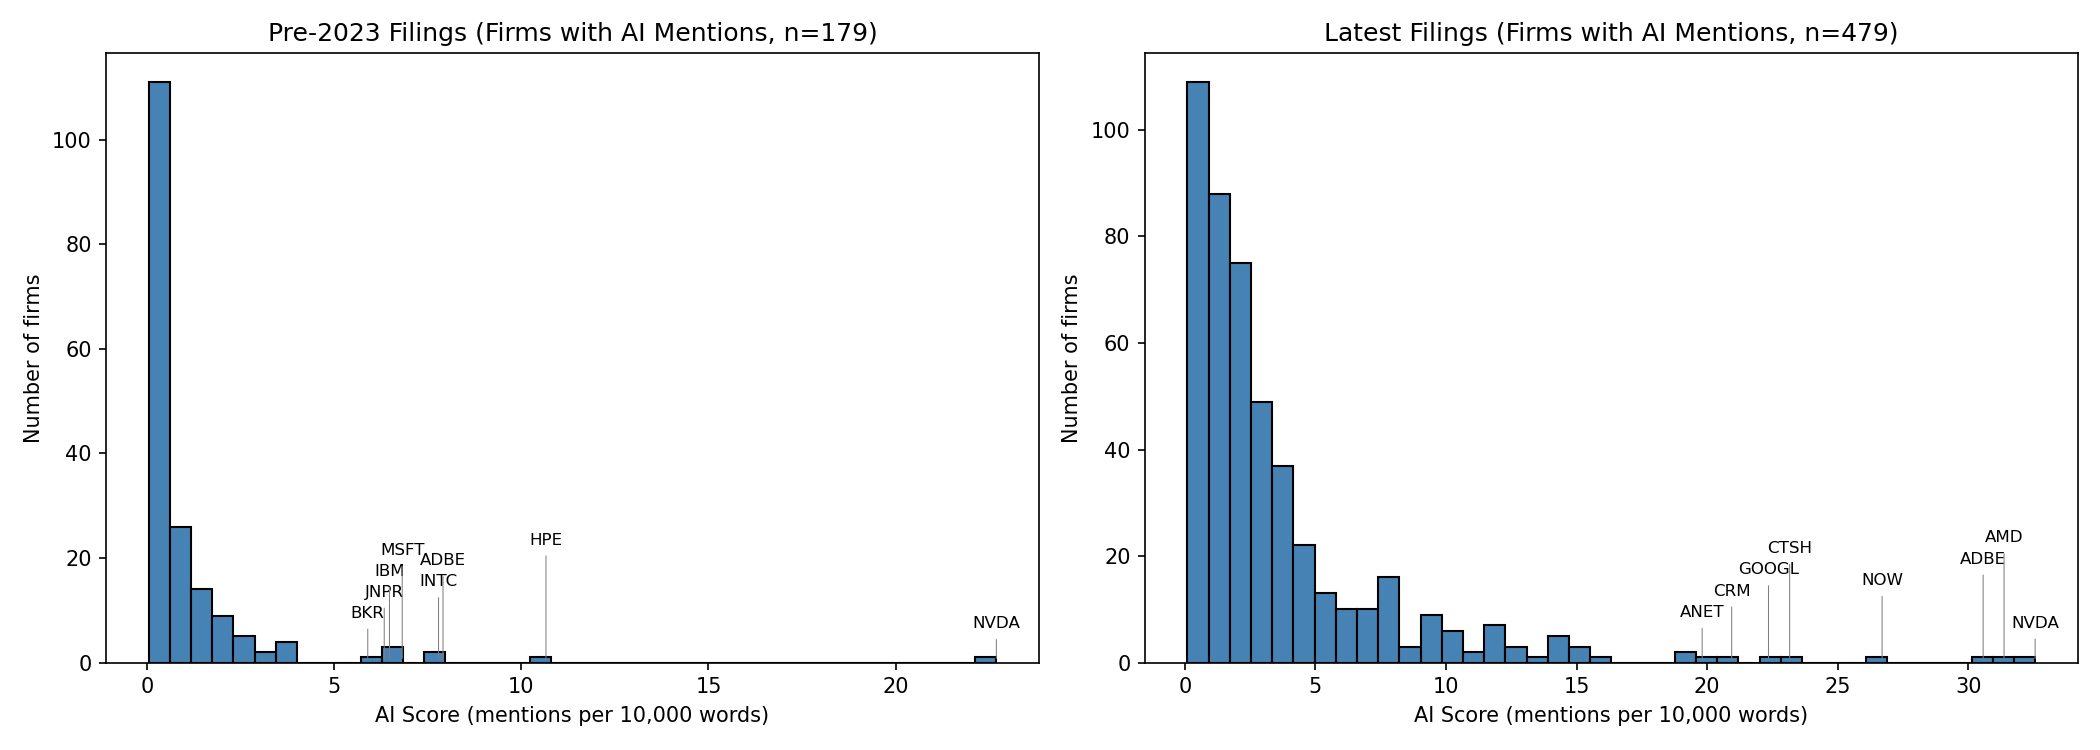
\includegraphics[width=\textwidth]{Pics/ai_score_comparison_pre_vs_post.png}
    \caption{Distribution of AI exposure scores among S\&P 500 firms with at least one AI-related keyword mention. The left panel shows scores based on the most recent 10-K filing available before 31 December 2022. The right panel shows scores from the most recent available filing. The number of firms mentioning AI increased from 179 to 479, and the distribution shifted substantially to the right, consistent with a broad-based increase in corporate AI disclosure following the release of ChatGPT}
\label{fig:ai_score_distribution}
\end{figure}


This skewness of the pre 2023 filings means that a standard quintile split, which would place roughly 100 firms in each group, produces three effectively identical bottom groups with average scores of zero. We instead assign firms to three groups based on the natural structure of the data. Firms with no AI-related mentions are classified as having No AI Exposure (319 firms). Among the 179 firms with at least one mention, those with a normalised score below the group median are classified as Moderate AI Exposure (87 firms), and those at or above the median as High AI Exposure (92 firms). This approach produces groups that are meaningfully distinct: the High group averages 12.4 AI mentions per filing with a mean normalised score of 2.00, the Moderate group averages 1.79 mentions with a score of 0.21, and the No Exposure group is identically zero.

\begin{table}[H]
\centering
\caption{Summary Statistics by AI Exposure Group}
\small
\setlength{\tabcolsep}{4pt}
\begin{tabular}{lccccc}
\toprule
Group & Firms & Mean AI & Median AI & Mean AI & Median AI \\
      &       & Mentions & Mentions & Score & Score \\
\midrule
High AI Exposure     & 92  & 12.20 & 7.0 & 1.97 & 1.06 \\
Moderate AI Exposure & 87  & 1.79  & 1.0 & 0.21 & 0.19 \\
No AI Exposure       & 319 & 0.00  & 0.0 & 0.00 & 0.00 \\
\midrule
Total                & 498 &      &     &      &      \\
\bottomrule
\end{tabular}
\vspace{0.4em}
\begin{minipage}{0.95\linewidth}
\footnotesize
\textit{Notes:} AI exposure score is measured as AI-related keyword mentions per 10{,}000 words in the latest 10-K filing available by 31 December 2022. Firms with zero AI mentions are classified as No AI Exposure. The remaining firms are split at the median normalized AI score into Moderate and High AI Exposure.
\end{minipage}

\end{table}

\subsection{Limitations}

Any text-based classification involves trade-offs, and the approach adopted here is no exception. Several limitations should be noted.

The keyword-based approach measures what firms disclose about AI, not what they actually do with it. Two notable cases illustrate this distinction. Apple is classified as having no AI exposure despite possessing significant internal machine learning capabilities, including its Siri voice assistant and on-device intelligence features. Netflix presents a similar case: its recommendation engine is one of the most prominent applications of machine learning in consumer technology, yet the company does not describe it in AI terms in its 10-K filings.

These cases point to a genuine limitation of the measure. Firms that invest heavily in AI but describe it in proprietary or non-standard language will be underrepresented. 

A second limitation concerns the coarseness of the keyword approach. The measure treats all mentions equally, whether a firm discusses AI as a core product, a future aspiration, or a risk factor. A company that warns about AI-related competitive threats in its risk disclosures receives the same score as one that describes AI as central to its revenue model.

Finally, the measure is limited to the eight keywords selected for the dictionary. While the expanded screening of 65 candidate terms suggests that the retained keywords capture the vast majority of relevant variation, it is possible that some firms describe AI related activities using terminology not included in the dictionary. 


\section{Theoretical Framework}

With the classification in place, we now have a tool that allows us to compare the market behaviour of firms with different levels of pre-boom AI engagement. The 92 firms in the High AI Exposure group, the 87 in the Moderate group, and the 319 firms with no AI-related mentions in their filings form the basis for the empirical tests that follow. Before turning to those tests, however, it is necessary to set out the theoretical framework that motivates them: what does it mean for asset prices to deviate from fundamentals, why might technology-driven booms produce such deviations, and how can we detect them in the data?

\subsection{Asset prices and fundamental value}

The starting point for any analysis of speculative excess is the present value model of asset pricing. Under standard assumptions, the price of an asset is determined by

\begin{equation}
P_t = \sum_{i=0}^{\infty} \left( \frac{1}{1+r_f} \right)^i E_t \left( D_{t+i} + U_{t+i} \right) + B_t,
\end{equation}

\noindent where $P_t$ is the asset price, $r_f$ is the risk-free rate, $D_t$ denotes the payoff (e.g., dividends), $U_t$ represents unobservable factors, and $B_t$ is a bubble component. When $B_t = 0$, the asset is priced according to fundamentals alone and the price series generally exhibits at most $I(1)$ behaviour. A speculative bubble arises when $B_0 > 0$, in which case the bubble component satisfies the submartingale property

\begin{equation}
E_t(B_{t+1}) = (1 + r_f) B_t.
\end{equation}

\noindent When $B_t$ is present, it tends to dominate price dynamics, transmitting explosive behaviour to the series $P_t$ (Phillips, Shi and Yu, 2015a).\footnote{Phillips, P.C.B., Shi, S., and Yu, J., ``Testing for Multiple Bubbles: Historical Episodes of Exuberance and Collapse in the S\&P 500,'' \textit{International Economic Review}, 56(4), 2015, pp.\ 1043--1078.} The bubble component is latent and not directly observable, but its presence can be inferred from the explosive dynamics it induces in the price series.

The efficient market hypothesis, as articulated by Fama (1970), holds that asset prices at all times fully reflect available information.\footnote{Fama, E.F., ``Efficient Capital Markets: A Review of Theory and Empirical Work,'' \textit{Journal of Finance}, 25(2), 1970, pp.\ 383--417.} In its strongest form, this implies that sustained mispricings should not occur, because rational arbitrageurs would immediately trade against any deviation from fundamental value. Under this view, the divergence in returns between High AI Exposure firms and the rest of the index, if it exists, would simply reflect a rational updating of expectations about the future earnings capacity of those firms.

Yet the historical record suggests that markets do not always price new technologies correctly. Shiller (2000) argued that financial markets are subject to waves of irrational exuberance, in which investor psychology, narrative contagion, and feedback trading drive prices above levels justified by careful analysis of fundamentals.\footnote{Shiller, R.J., \textit{Irrational Exuberance}, Princeton University Press, 2000.} When the ultimate economic impact of a new technology is genuinely unknown, even well-informed investors face a valuation problem that rational models struggle to resolve. It is precisely this uncertainty that creates room for the bubble component $B_t$ to emerge.

\subsection{Technology and speculation: a recurring pattern}

The link between technological innovation and speculative excess is one of the most persistent features of financial history. Kindleberger and Aliber (2015) document a recurring sequence: a displacement, typically a new technology or financial innovation, triggers a period of rising asset prices, which attracts additional capital, loosens credit conditions, and eventually produces a self-reinforcing cycle of enthusiasm that overshoots any plausible estimate of fundamental value.\footnote{Aliber, R.Z., Kindleberger, C.P., and McCauley, R.N., \textit{Manias, Panics, and Crashes: A History of Financial Crises}, Springer, 2015.}

The specific technologies change, but the pattern is remarkably stable. In the 1920s, the Radio Corporation of America (RCA) became a focal point for investor enthusiasm about radio broadcasting; its stock rose from roughly \$94 to \$505 between early 1928 and September 1929, substantially outpacing the company's actual sales performance, before collapsing in the crash of October 1929.\footnote{Bruner, R.F. and Miller, S.C., ``The Great Crash of 1929: A Look Back After 90 Years,'' \textit{Journal of Applied Corporate Finance}, 31(4), 2019, pp.\ 43--58; Sirkin, G., ``The Stock Market of 1929 Revisited: A Note,'' \textit{Business History Review}, 49(2), 1975, pp.\ 223--231.} The dot-com boom of the late 1990s followed a similar arc: Cisco, the largest networking company on the Nasdaq, peaked at \$132 in March 2000 before declining to \$16 within a year.\footnote{Hirschey, M., ``Cisco and the Kids (corrected),'' \textit{Financial Analysts Journal}, 57(4), 2001, pp.\ 48--59.}

P\'{a}stor and Veronesi (2009) provide a theoretical account of why technology generates this pattern.\footnote{P\'{a}stor, L. and Veronesi, P., ``Technological Revolutions and Stock Prices,'' \textit{American Economic Review}, 99(4), 2009, pp.\ 1451--1483.} They show that the arrival of a major new technology increases uncertainty about the future productivity of firms, which initially raises both the level and the volatility of asset prices. As information about the technology's true impact is gradually revealed, prices adjust, sometimes sharply downward. Importantly, this framework demonstrates that large price run-ups can occur even without irrational behaviour: genuine uncertainty about a transformative technology is itself sufficient to produce price dynamics that resemble a bubble ex post. Whether any specific episode reflects rational uncertainty pricing or speculative excess must therefore be assessed with data.

\subsection{The productivity paradox and the lag problem}

A central difficulty in evaluating whether AI valuations are justified is that transformative technologies often take far longer to generate measurable economic returns than initial market enthusiasm implies. This problem was formalised by Brynjolfsson (1993) as the ``productivity paradox'' of information technology: despite massive investment in computing power from the 1970s onward, aggregate productivity statistics showed little improvement.\footnote{Brynjolfsson, E., ``The Productivity Paradox of Information Technology: Review and Assessment,'' \textit{Communications of the ACM}, December 1993.} As Robert Solow famously remarked, computers could be seen everywhere except in the productivity statistics.

Brynjolfsson identified several possible explanations for this gap: measurement errors in output statistics, lags between investment and the organisational changes required to exploit new technology, redistribution of rents rather than creation of new value, and mismanagement. The most analytically important of these is the lag hypothesis. Drawing on an analogy to the electrification of factories, David (1990) showed that major productivity gains from electric power did not materialise for roughly two decades, because the full benefits required redesigning production processes around the new technology.\footnote{David, P.A., ``The Dynamo and the Computer: An Historical Perspective on the Modern Productivity Paradox,'' \textit{American Economic Review}, 80(2), 1990, pp.\ 355--361.}

This insight connects directly to the CAPEX dynamics documented in section 1.2 and to the classification constructed above. The firms in the High AI Exposure group are, by construction, the firms that were already discussing AI as a meaningful part of their business before the boom. If AI follows the trajectory suggested by the productivity paradox literature, then the productivity gains that justify these firms' current valuations may not materialise for years, even if the technology ultimately proves transformative. The gap between current investment and future payoff is precisely the space in which the bubble component $B_t$ can develop.

\subsection{Detecting bubbles: from theory to econometrics}

The theoretical frameworks reviewed above establish that speculative excess is plausible in the current environment but do not, on their own, determine whether it is actually present. Answering that question requires econometric tools that can distinguish between prices rising because of improving fundamentals and prices exhibiting the explosive dynamics characteristic of a speculative bubble.

The key methodological advance was developed by Phillips, Wu and Yu (2011) and refined in Phillips, Shi and Yu (2015a, 2015b).\footnote{Phillips, P.C.B., Wu, Y., and Yu, J., ``Explosive Behavior in the 1990s Nasdaq: When Did Exuberance Escalate Asset Values?'' \textit{International Economic Review}, 52(1), 2011, pp.\ 201--226.}\footnote{Phillips, P.C.B., Shi, S., and Yu, J., ``Testing for Multiple Bubbles: Limit Theory of Real-Time Detectors,'' \textit{International Economic Review}, 56(4), 2015, pp.\ 1079--1134.} Their approach, the PSY procedure, is built on the following framework. Let $y_t$ be a dividend-adjusted price series. Under the null hypothesis of no bubble, the series satisfies

\begin{equation}
y_t = dT^{-\eta} + y_{t-1} + \varepsilon_t, \qquad \varepsilon_t \sim \text{iid}(0, \sigma^2),
\end{equation}

\noindent where $d$ is a constant, $T$ is the sample size, and $\eta$ is a localising coefficient that accommodates an asymptotically negligible drift when $\eta > 1/2$. Under this specification, the price follows a unit root process consistent with fundamentals-driven pricing.

The alternative hypothesis of bubble presence is given by mildly explosive dynamics (Phillips and Magdalinos, 2007):\footnote{Phillips, P.C.B. and Magdalinos, T., ``Limit Theory for Moderate Deviations from a Unit Root,'' \textit{Journal of Econometrics}, 136(1), 2007, pp.\ 115--130.}

\begin{equation}
y_t = \theta_T y_{t-1} + \varepsilon_t,
\end{equation}

\noindent where the autoregressive parameter $\theta_T$ exceeds unity:

\begin{equation}
\theta_T = 1 + \frac{c}{T^{\alpha}}, \qquad \alpha \in (0,1), \quad c > 0.
\end{equation}

\noindent When $\theta_T > 1$, the price series exhibits explosive behaviour, growing at a rate that exceeds what a unit root process would imply. The PSY procedure tests for this explosive behaviour using a sequence of right-tailed augmented Dickey--Fuller (ADF) statistics computed over recursive subsamples of the data. The backward sup ADF (BSADF) statistic for each observation is

\begin{equation}
\text{BSADF}_t(\tau_0) = \sup_{\tau_1 \in [0, \, t - \tau_0]} \left\{ \text{ADF}_{\tau_1}^{t} \right\},
\end{equation}

\noindent where $\tau_0$ is the minimum window size and $\text{ADF}_{\tau_1}^{t}$ is the ADF $t$-statistic estimated on the subsample from $\tau_1$ to $t$. The generalised sup ADF (GSADF) statistic is then

\begin{equation}
\text{GSADF}(\tau_0) = \sup_{\tau \in [\tau_0, \, 1]} \left\{ \text{BSADF}_\tau(\tau_0) \right\}.
\end{equation}

\noindent Under the null hypothesis, the GSADF statistic has a known limiting distribution. Rejection of the null in favour of the explosive alternative provides evidence of bubble-like dynamics in the price series. The procedure also allows for date-stamping: a bubble is identified as originating at the first observation where the BSADF statistic exceeds the corresponding critical value sequence, and as terminating when it falls back below.

This methodology has been applied to equity markets, bond markets, commodities, and real estate.\footnote{See, among others, Phillips and Shi (2018) on stock markets, Etienne et al.\ (2015) on commodities, Caspi et al.\ (2018) on oil prices, and Pavlidis et al.\ (2016) on housing markets. The Federal Reserve Bank of Dallas uses a version of the PSY procedure to monitor global housing market exuberance in real time.} Basele, Phillips and Shi (2025) have recently applied these methods to the Nasdaq and the Magnificent Seven during the current AI boom, finding evidence of speculative bubbles in the Nasdaq index and across six of the seven stocks from December 2022 to January 2025.\footnote{Basele, R.B., Phillips, P.C.B., and Shi, S., ``Speculative Bubbles in the Recent AI Boom: Nasdaq and the Magnificent Seven,'' Cowles Foundation Discussion Paper No.\ 2430, Yale University, March 2025.}

\subsection{From theory to empirical strategy}

The theoretical framework presented in this section rests on four pillars. First, the present value identity in equation (1) provides a formal definition of a speculative bubble as a deviation of market prices from their fundamental value, captured by a non-zero bubble component $B_t$ satisfying the submartingale condition in equation (2). Second, the historical literature on technology-driven speculation shows that new technologies routinely trigger asset price dynamics that exceed what fundamentals can support. Third, the productivity paradox highlights that the economic benefits of transformative technologies may lag behind their market impact by years or decades, creating a structural gap between investor expectations and realised returns in which $B_t$ can emerge. Fourth, the PSY framework provides a formal statistical test for the explosive dynamics in equations (4)--(5) that characterise speculative episodes.

These four pillars motivate the empirical analysis that follows. The AI exposure classification constructed in section 1 allows us to move beyond market-level tests and ask a more specific question: has the post-2022 repricing of AI-exposed firms been proportionate to their fundamentals, or does it exhibit the patterns that the literature associates with speculative excess? We begin by examining return differentials across the three exposure groups and testing whether observable firm characteristics can account for the divergence. We then turn to formal tests for explosive dynamics in the price series of AI-exposed firms.

\end{document}